
% Setting up the document class for presentation
\documentclass[11pt]{beamer}

% Including essential packages
\usepackage[utf8]{inputenc}
\usepackage[T1]{fontenc}
\usepackage{lmodern}
\usepackage{xcolor}
\usepackage{hyperref}
\usepackage{graphicx}

% Defining theme and colors
\usetheme{metropolis}
\definecolor{primary}{RGB}{0, 102, 204}
\definecolor{secondary}{RGB}{255, 153, 51}
\setbeamercolor{frametitle}{bg=primary, fg=white}
\setbeamercolor{normal text}{fg=black}
\setbeamerfont{title}{size=\large}
\setbeamerfont{frametitle}{size=\normalsize}

% Configuring fonts (using a clean sans-serif font)
\usepackage[sfdefault]{lmodern} % Fallback sans-serif font

% Title slide information
\title{Pose Recognition Web App}
\subtitle{AI-Powered Real-Time Pose Detection with Local Model Support}
\author{Replit Development Team}
\date{July 09, 2025}

\begin{document}

% Creating title slide
\begin{frame}
    \titlepage
\end{frame}

% Overview
\begin{frame}{What is Pose Recognition App?}
    \begin{itemize}
        \item \textbf{Real-time pose detection} using webcam input
        \item \textbf{Offline functionality} - no internet required after setup
        \item \textbf{Customizable settings} for 1-7 poses
        \item \textbf{Local model support} with Teachable Machine integration
        \item \textbf{Distance calibration} for optimal positioning
        \item \textbf{Audio feedback} and visual guidance
    \end{itemize}
\end{frame}

% Core Features
\begin{frame}{Core Features}
    \begin{block}{Pose Recognition System}
        \begin{itemize}
            \item Support for 1-7 customizable poses
            \item Real-time confidence scoring (30-90\% threshold)
            \item Visual pose comparison with reference images
            \item Skeletal tracking with 17 keypoints
        \end{itemize}
    \end{block}
    \begin{block}{Customization Options}
        \begin{itemize}
            \item Adjustable recognition delay (1-10 seconds)
            \item Custom pose names (editable labels)
            \item Audio beep toggle for success feedback
            \item Distance calibration with real-time guidance
        \end{itemize}
    \end{block}
\end{frame}

% GUI: Settings Interface
\begin{frame}{GUI: Settings Interface}
    \begin{center}
        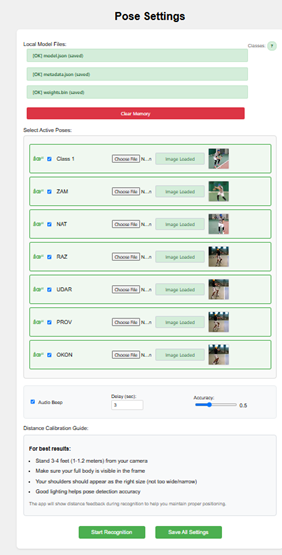
\includegraphics[width=0.7\textwidth]{GUI1_1752049448296.png}
    \end{center}
    \small{
    \textbf{Key Features:}
    \begin{itemize}
        \item Local model file uploads (model.json, metadata.json, weights.bin)
        \item Pose selection checkboxes for 1-7 poses
        \item Reference image uploads for each pose
        \item Audio, delay, and accuracy threshold controls
        \item Distance calibration guide
    \end{itemize}
    }
\end{frame}

% GUI: Recognition Interface
\begin{frame}{GUI: Recognition Interface}
    \begin{center}
        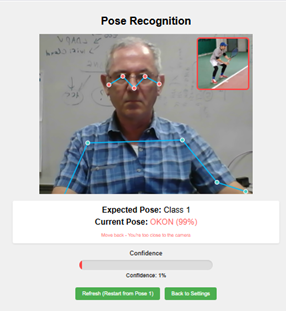
\includegraphics[width=0.7\textwidth]{GUI2_1752049449853.png}
    \end{center}
    \small{
    \textbf{Real-time Features:}
    \begin{itemize}
        \item Live webcam feed with pose detection
        \item Current vs Expected pose display
        \item Confidence bar with color coding (green = correct, red = incorrect)
        \item Reference image comparison
        \item Refresh and back to settings controls
    \end{itemize}
    }
\end{frame}

% Technical Specifications
\begin{frame}{Technical Specifications}
    \begin{block}{AI Framework}
        \begin{itemize}
            \item TensorFlow.js with Teachable Machine models
            \item PoseNet for 17-keypoint skeletal tracking
            \item Local storage with IndexedDB for offline use
        \end{itemize}
    \end{block}
    \begin{block}{Compatibility}
        \begin{itemize}
            \item Modern browsers with WebRTC support
            \item Optimized for Windows compatibility
            \item Automatic image compression for storage
            \item Multiple camera resolution fallback
        \end{itemize}
    \end{block}
\end{frame}

% Setup Process
\begin{frame}{Easy Setup Process}
    \begin{enumerate}
        \item \textbf{Train Your Model:} Use Teachable Machine to create pose model
        \item \textbf{Upload Files:} Import model.json, metadata.json, weights.bin
        \item \textbf{Configure Poses:} Select 1-7 poses and upload reference images
        \item \textbf{Adjust Settings:} Set audio, delay, and accuracy preferences
        \item \textbf{Start Recognition:} Begin real-time pose detection
    \end{enumerate}
    \vspace{0.5cm}
    \begin{alertblock}{Fully Offline}
        Works completely without internet after initial setup
    \end{alertblock}
\end{frame}

% Advanced Features
\begin{frame}{Advanced Features}
    \begin{block}{Distance Calibration}
        \begin{itemize}
            \item Auto-detection of user distance from camera
            \item Real-time feedback for optimal positioning (3-4 feet)
            \item Visual cues: Green = perfect, Red = adjust distance
        \end{itemize}
    \end{block}
    \begin{block}{Data Management}
        \begin{itemize}
            \item Save all settings and model files locally
            \item Clear memory function with confirmation
            \item Auto-save for pose selections and custom names
            \item Persistent settings across browser sessions
        \end{itemize}
    \end{block}
\end{frame}

% Use Cases
\begin{frame}{Use Cases}
    \begin{itemize}
        \item \textbf{Fitness Training:} Monitor exercise form and technique
        \item \textbf{Yoga Practice:} Guide through pose sequences with feedback
        \item \textbf{Physical Therapy:} Track rehabilitation exercises
        \item \textbf{Sports Coaching:} Analyze athletic movements
        \item \textbf{Education:} Teach proper posture and movement
        \item \textbf{Accessibility:} Assistive technology for movement training
    \end{itemize}
\end{frame}

% Benefits
\begin{frame}{Key Benefits}
    \begin{block}{Privacy & Security}
        \begin{itemize}
            \item No data sent to external servers
            \item Local processing ensures privacy
            \item Offline functionality protects user data
        \end{itemize}
    \end{block}
    \begin{block}{User Experience}
        \begin{itemize}
            \item Instant feedback with audio and visual cues
            \item Customizable difficulty and timing
            \item Clear progress tracking through pose sequences
        \end{itemize}
    \end{block}
\end{frame}

% Get Started Today!
\begin{frame}{Get Started Today!}
    \begin{center}
        \Large Transform your training experience with\\
        \textbf{Pose Recognition Web App}\\
        \vspace{0.5cm}
        \normalsize
        \textbf{Available on Replit:} Easy deployment and sharing\\
        \textbf{Open Source:} Customizable for your needs\\
        \textbf{No Installation:} Run directly in your browser
    \end{center}
    \begin{block}{Ready to Use}
        \begin{itemize}
            \item Deploy instantly on Replit
            \item Share with your team or students
            \item Customize for specific use cases
        \end{itemize}
    \end{block}
\end{frame}

\end{document}
